% !TeX root = ../../main.tex
\subsection{磁铁性能评价}
\label{magnet_performance}
磁铁的剩余磁化强度越大越有利于捕捉井筒中的铁磁性颗粒物，本课题对磁铁的设计目标是

\begin{figure}[htbp]
	\centering
	\subfloat[实验装置结构及原理]{%
	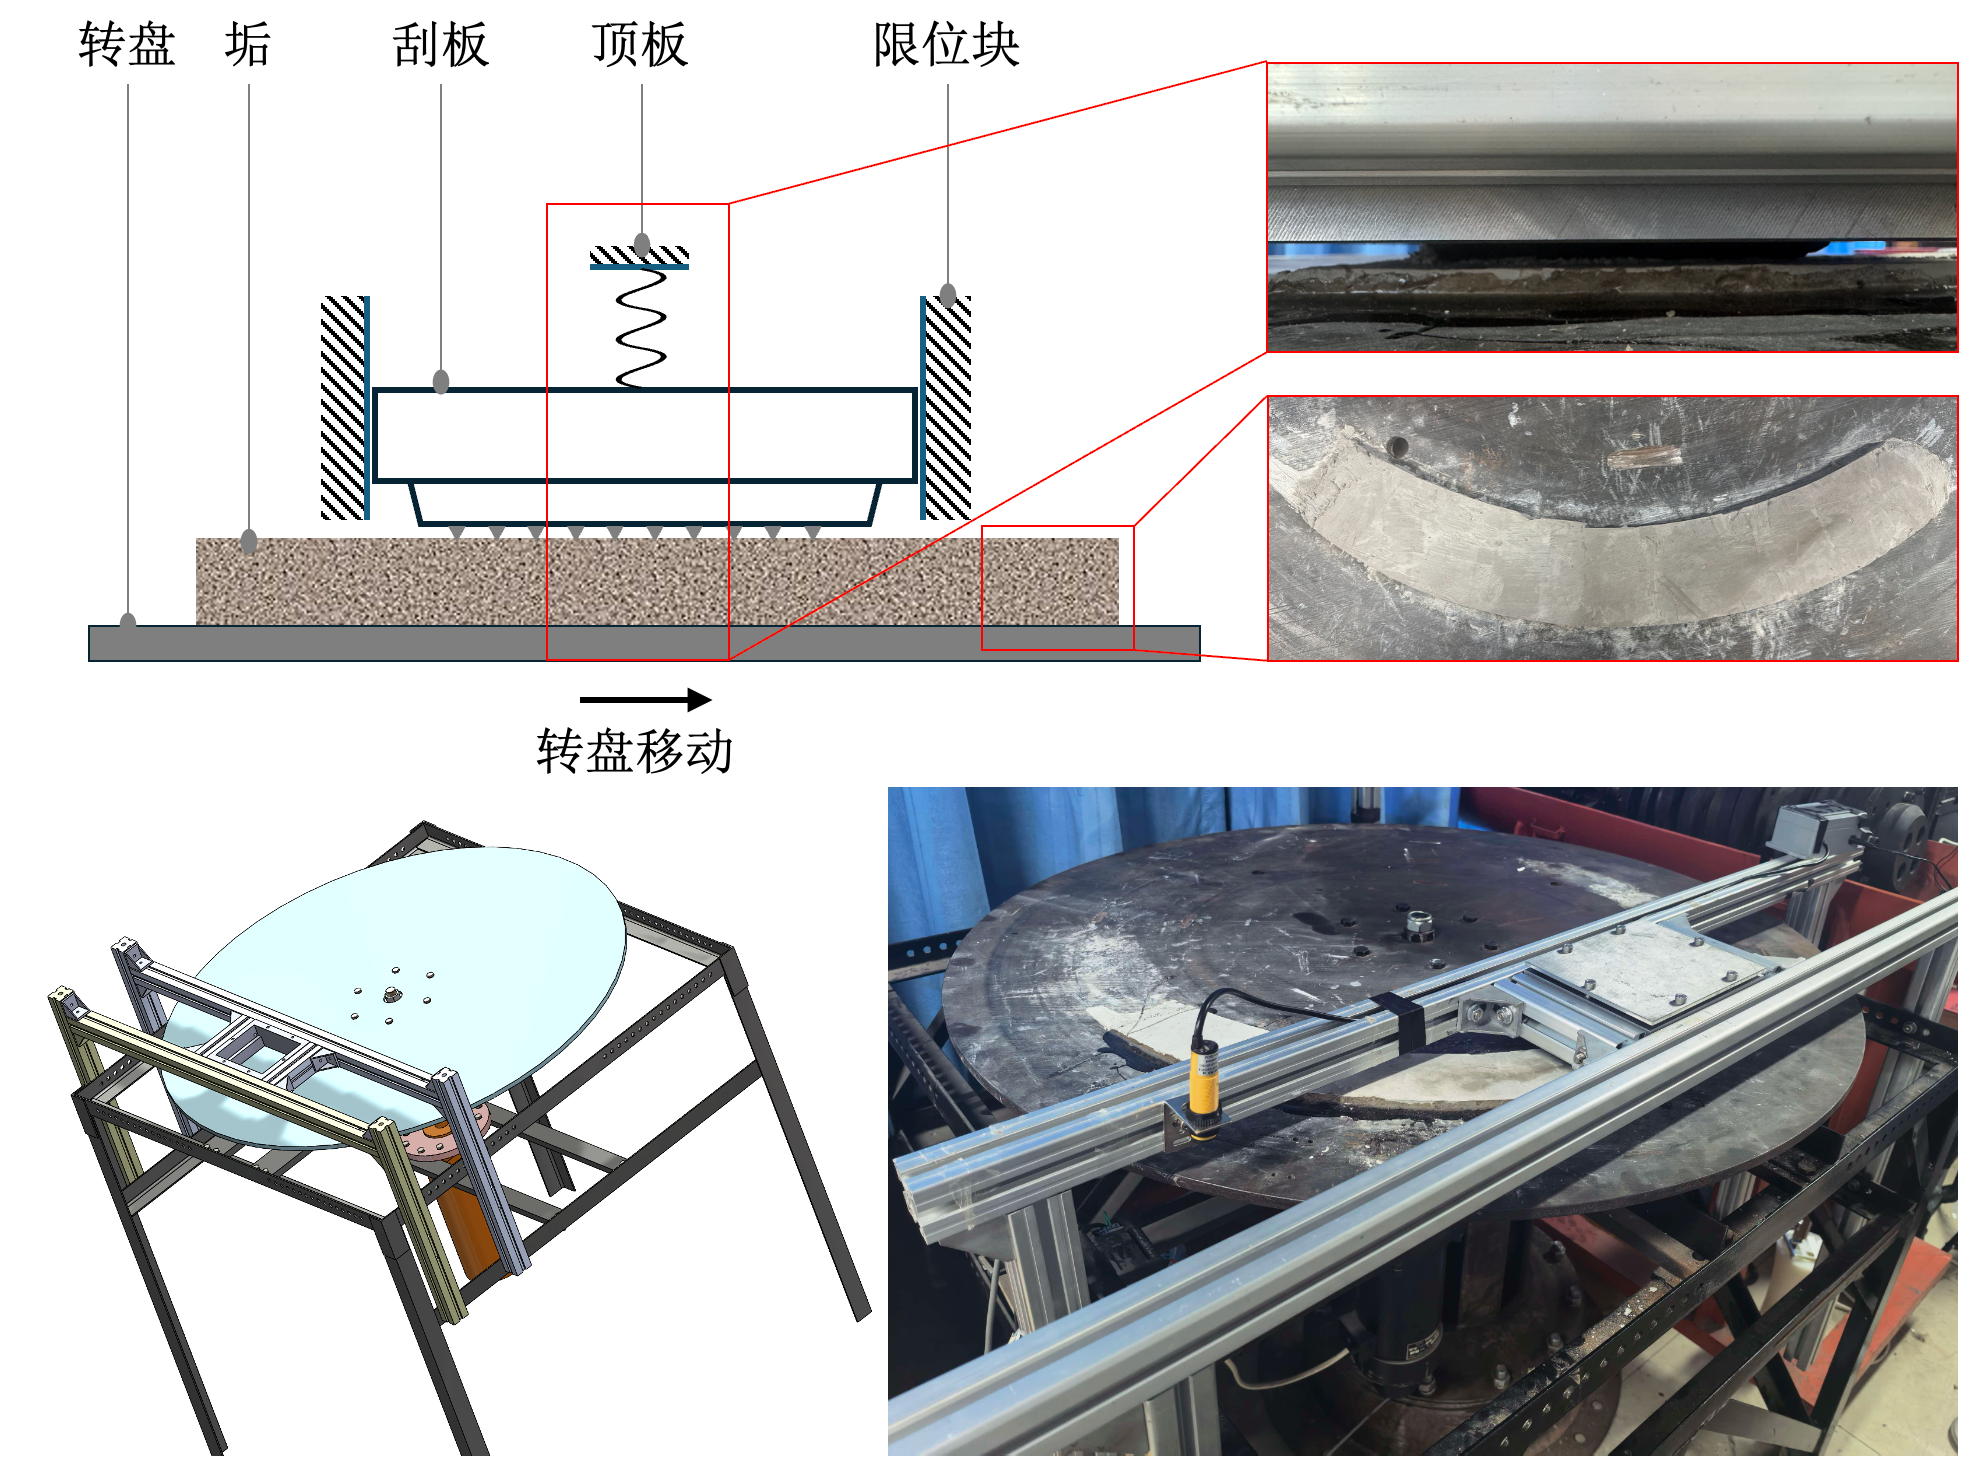
\includegraphics[width=.9\textwidth]{figure/chapter3/scraper-test-rig.png}
	\label{fig:scraper_test_rig_mechanism}
	}
	\vspace{1em}
	\subfloat[弹簧变形量测量原理]{%
	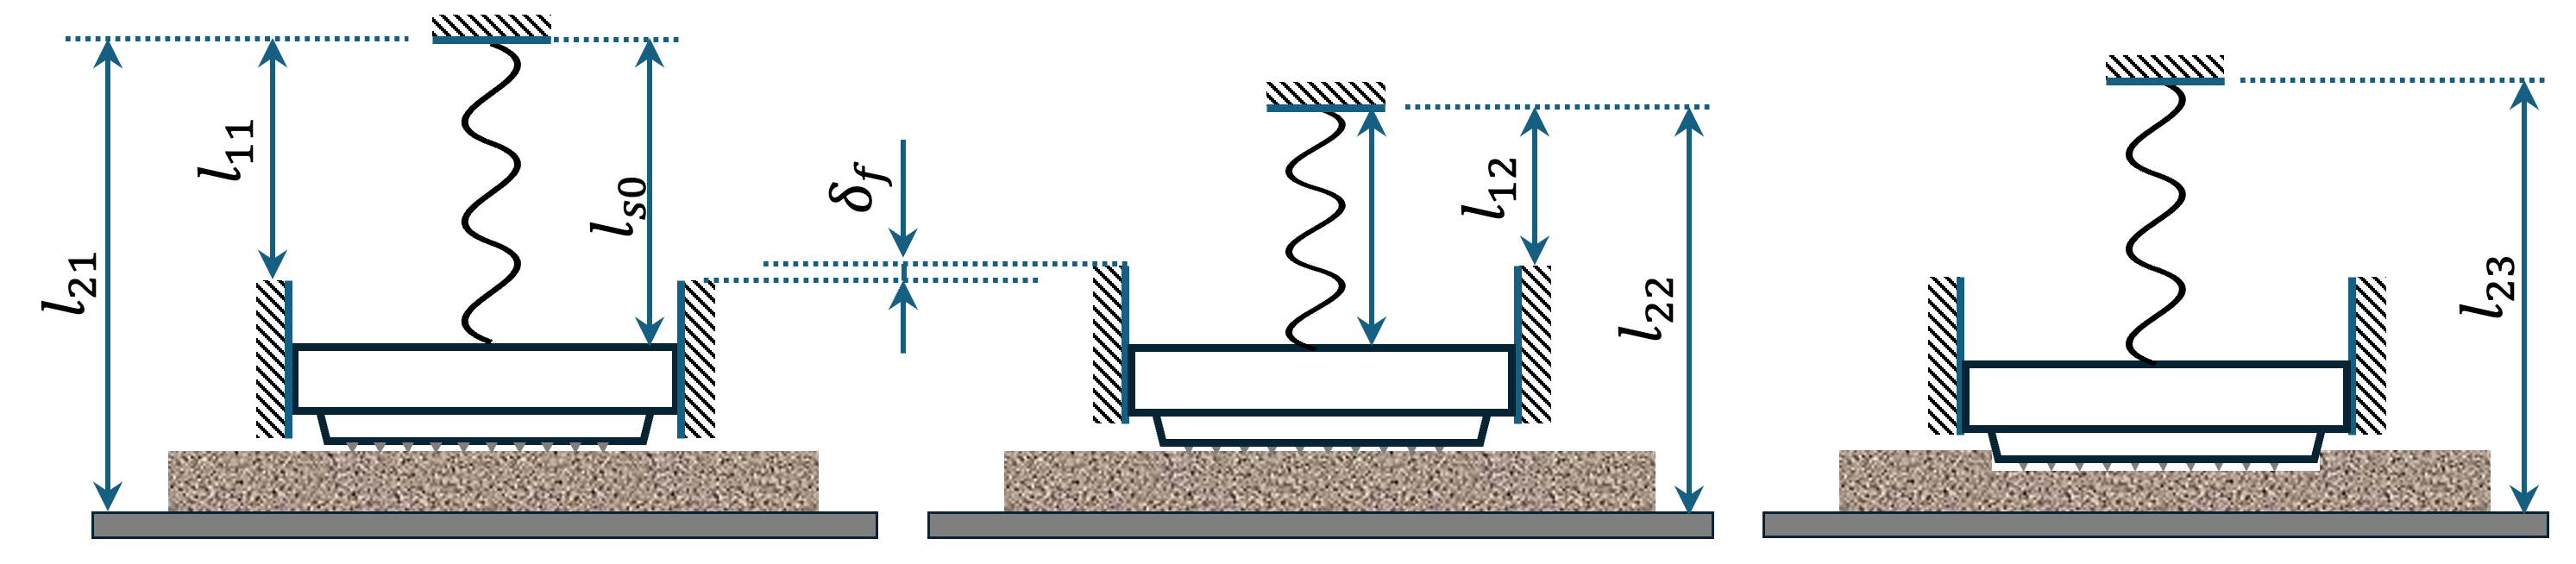
\includegraphics[width=.9\textwidth]{figure/chapter3/scapter-measurement-mechanism.png}
	\label{fig:scapter_measurement_mechanism}
	}
	\caption{刮板刮削性能测试}
	\label{fig:scraper_test_rig}
\end{figure}

。

